\chapter{Teoria cinetica dei gas}


\section{Modello dei gas ideali}
Nella realt\`a i gas sono composti da tante particelle. Imponiamo alcune condizioni che ci aspettiamo dai gas:
\setlength{\leftmargini}{0cm}
\begin{itemize}
\item[$\boxed{\text{Isotropo}}$] Le velocit\`a delle particelle sono equamente distribuite in ogni direzione.
\item[$\boxed{\text{Omogeneo}}$] Le particelle sono equamente distribuite.
\end{itemize}
\setlength{\leftmargini}{0.5cm}
Sia $dn(v)$ il numero di particelle con una data velocit\`a.
\begin{remark}
Se $N$ \`e il numero totale di particelle
\[N=\int dn(v)=\int_0^\infty \dd vndv\]
dove $\dd vn$ \`e in un qualche modo la ``densit\`a delle particelle di una data velocit\`a".
\end{remark}

\begin{definition}[Angolo solido]
Definiamo l'\textbf{angolo solido} relativo ad un isieme di vettori $\cpa{\vec u}$ come l'area di $S^2$ occupata da $\cpa{\frac{\vec u}{\abs{\vec u}}}$.\\
Il differenziale dell'angolo solido \`e 
\[d\Omega=\sin\theta d\theta d\phi\]
\end{definition}

\begin{definition}[Velocit\`a quadratica media]
Definiamo la \textbf{velocit\`a quadratica media delle particelle} come
\[\ps{v^2}=\int_0^\infty v^2dn(v)\] 
\end{definition}

\begin{definition}[Energia cinetica media]
Definiamo l'\textbf{energia cinetica media} come \[\ps{E_K}=\frac12mN\ps{v^2}.\]
\end{definition}

\begin{proposition}[Calcolo della pressione]\label{CalcoloDellaPressioneTeoriaCineticaDeiGas}
Sia $m$ la massa di una particella, $N$ il numero di particelle e $V$ il volume che occupano. La pressione collettiva che queste particelle esercitano \`e
\[p=\frac13m\frac NV\ps{v^2}.\]
\end{proposition}
\begin{proof}
Calcoliamo qualche differenziale utile
\setlength{\leftmargini}{0cm}
\begin{itemize}
\item[$\boxed{dn(\vec v)}$] Sia $\vec v$ una qualche velocit\`a.
\[dn(\vec v)\pasgnl={isotropia}dn(v)\frac{d\Omega}{4\pi},\]
dove $d\Omega$ \`e il differenziale dell'angolo solido occupato dalle possibili velocit\`a. 
\item[$\boxed{dn}$] Per omogeneit\`a il numero di particelle in un volumetto \`e
\[dn=\frac NVdV=\frac NV dAvdt\cos\theta.\]
\begin{figure}[!htb]
    \centering
    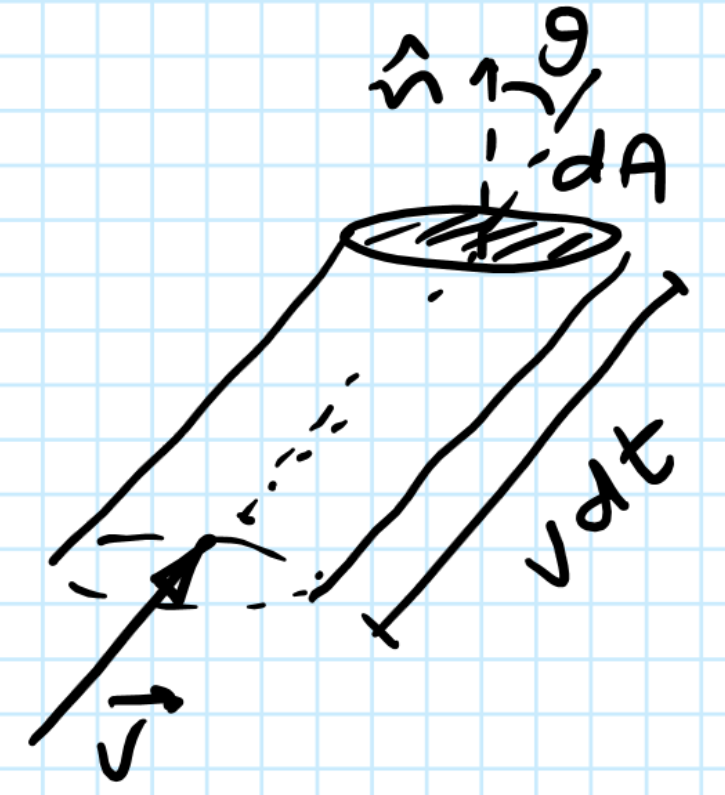
\includegraphics[width=3cm]{images/volumetto_per_impulso_infinitesimo.png}
\end{figure}
\end{itemize}
\setlength{\leftmargini}{0.5cm}
Assumendo impatti elatici, l'impulso trasferito alla parete dall'impatto di una particella \`e $\abs{\Delta \vec p}=2mv\cos \theta$.\medskip

\noindent Appurate queste equazioni possiamo scrivere il differenziale della pressione come segue:
\begin{align*}
d^2p=&\frac{dF}{dA}=\frac{\abs{d\vec p}/dt}{dA}=\frac1{dA}\frac1{dt}\abs{d\vec p}_{singola}dn dn(\vec v)\\
=&\frac1{dA}\frac1{dt}{2mv\cos \theta}\quad{\frac{N}V dAvdt\cos \theta}\quad{dn(v)\frac{d\Omega}{4\pi}}=\\
=&N\frac{2mv^2\cos^2\theta}Vdn(v)\frac{d\Omega}{4\pi}.
\end{align*}
Facendo la media su tutte le direzioni troviamo il vero differenziale della pressione:
\begin{align*}
dp=&\int_\Omega d^2p=\frac{mv^2}{2\pi}\frac NVdn(v)\int_0^{2\pi}d\phi\int_0^{\pi/2}\cos^2\theta\sin\theta d\theta=\\
=&\frac13mv^2\frac NVdn(v).
\end{align*}
Integrando ora sui possibili moduli delle velocit\`a troviamo la pressione:
\[p=\frac13m\frac NV\ps{v^2}\int_0^\infty v^2dn(v)=\frac13m\frac NV\ps{v^2}.\]
\end{proof}


\begin{proposition}
Per gas ideali vale la relazione
\[\boxed{\ps{E_K}=\frac32 k_b T}\]
\end{proposition}
\begin{proof}
Osserviamo che
\[pV=\frac13 mN\ps{v^2},\]
dunque
\[nRT=pV=\frac13 mN\ps{v^2}=\frac23\ps{E_K},\]
cio\`e
\[T=\frac 23\frac{\ps{E_K}}{nR}=\frac 23N_a\frac{\ps{E_K}}{NR}=\frac 23\frac{\ps{E_K}}{Nk_b}\]
In conclusione
\[\ps{E_K}=\frac32 k_b T.\]
\end{proof}

\noindent
Consideriamo ora l'energia interna di questo sistema\footnote{affermare che $U=\ps{E_K}$ corrisponde ad assumere che il gas sia monoatomico.}:
\[U=\ps{E_K}=\frac32nRT=C_VT.\]
In generale $U=E_K+E_P$ per una qualche energia potenziale $E_P$. Per piccoli spostamenti $E_P=(E_P)_0+\frac12kx^2$\ \footnote{regime ragionevole per il tipo di forze che agisce all'interno di materiali.}. Nel caso biatomico per esempio $E_P=\frac12I\omega^2$.
\setlength{\leftmargini}{0cm}
\begin{itemize}
\item[$\boxed{\text{Solido}}$] 6 gradi di libert\`a: 3 potenziali (forze elastiche) e 3 cinetiche.
\item[$\boxed{\text{Gas perf. mono.}}$] 3 gradi di libert\`a, tutti cinetici.
\item[$\boxed{\text{Gas perf. bi.}}$] 5 gradi di libert\`a: 3 cinetici e 2 dalla rotazione \footnote{la rotazione lungo l'asse che congiunge le particelle \`e irrilevante}.
\end{itemize}
\setlength{\leftmargini}{0.5cm}


\begin{fact}[Principio di equipartizione]
Ogni grado di libert\`a contribuisce un addendo $\frac12 RT$ al calore specifico a volume costante.
\end{fact}

\begin{remark}
Abbiamo ricavato nuovamente l'espressione per $c_V$ che avevamo assunto per gas ideali:\\
Se le particelle hanno $\nu$ gradi di libert\`a allora
\[c_V=\frac\nu2RT.\]
\end{remark}

\section{Distribuzione di Maxwell-Boltzmann}
Consideriamo ora un sistema isolato con temperatura costante. Cerchiamo di capire come \`e fatta la distribuzione delle velocit\`a.\medskip

\noindent
Decomponiamo le velocit\`a $\vec v$ in $(v_x,v_y,v_z)$. Notiamo che
\[dn(v_x)=Nf(v_x)dv_x,\]
dove $f$ \`e la densit\`a di probabilit\`a che la componente $x$ sia $v_x$.\\
Per isotropia si ha che
\[dn(v_y)=Nf(v_y)dv_y,\quad dn(v_z)=Nf(v_z)dv_z,\]
dunque
\[dn(\vec v)=N f(v_x)f(v_y)f(v_z)dv_xdv_ydv_z.\]
Sempre per isotropia, in realt\`a $f(v_x)f(v_y)f(v_z)$ \`e una funzione $\phi(v)$ del modulo $v=\sqrt{v_x^2+v_y^2+v_z^2}$, non delle singole componenti.\bigskip

\noindent
Segue dunque che
\[\phi(v)=f(v_x)f(v_y)f(v_z)=f(v)f(0)f(0).\]
Dividendo per $f(0)^3$ troviamo
\[\frac{f(v)}{f(0)}=\frac{f(v_x)}{f(0)}\frac{f(v_y)}{f(0)}\frac{f(v_z)}{f(0)},\]
da cui passando ai logaritmi
\[\log\frac{f(v)}{f(0)}=\log \frac{f(v_x)}{f(0)}+\log\frac{f(v_y)}{f(0)}+\log\frac{f(v_z)}{f(0)}.\]
Per semplicit\`a notazionale sia $G(v)=\log\frac{f(v)}{f(0)}$, da cui
\[G(v)=G(v_x)+G(v_y)+G(v_z).\]
Derivando ora per $v_i$ con $i\in\cpa{x,y,z}$ troviamo
\[\frac{G'(v)v_i}v=G'(v_i),\]
da cui
\[\frac{G'(v)}{v}=\frac{G'(v_x)}{v_x}=\frac{G'(v_y)}{v_y}=\frac{G'(v_z)}{v_z}\doteqdot -2\al\]
Poich\'e $\al$ non dipende da $v_i$ possiamo integrare l'equazione sopra per trovare
\[G(v_i)=-\al v_i^2+C\]
che ricordando la definizione di $G$ significa che esiste $a>0$ tale che
\[f(v_i)=ae^{-\al v_i^2}.\]
Sostituendo questo nella definizione di $\phi$ si ha
\[\phi(v)=Ae^{-\al (v_x^2+v_y^2+v_z^2)}=Ae^{-\al v^2}.\]
Poich\'e $\phi$ \`e una densit\`a di probabilit\`a\footnote{abbiamo usato il fatto che $\int_{-\infty}^{+\infty}e^{-\al x^2}dx=\sqrt{\frac{\pi}\al}$} si ha che $A=\pa{\frac{\al}\pi}^{3/2}$, cio\`e
\[dn(\vec v)=N\pa{\frac{\al}\pi}^{3/2}e^{-\al v^2} dv_xdv_ydv_z.\]
Se ora integriamo sull'angolo solido troviamo il numero di particelle con una data velocit\`a:
\begin{align*}
dn(v)=&\int_\Omega dn(\vec v)=N\int_\Omega \phi(v)dv_xdv_ydv_z=\\
=&N\int_\Omega \phi(v)v^2dvd\Omega=\\
=&4\pi N\phi(v)v^2dv=\\
=&4N\sqrt{\frac{\al^3}\pi}v^2e^{-\al v^2}dv.
\end{align*}
Cerchiamo ora di capire chi \`e $\al$. Ricordiamo che 
\[\frac{3k_bT}m=\ps{v^2}=\frac{\int_0^\infty v^2dn(v)}{\int_0^\infty dn(v)}.\]
Sviluppando il termine di destra tramite identit\`a note sulla funzione Gamma\footnote{$\int_0^\infty x^ne^{-\al x^2}=\frac{\Gamma((n+1)/2)}{2a^{(n+1)/2}}$} ricaviamo
\[\int_0^\infty 4N\sqrt{\frac{\al^3}\pi} v^4e^{-\al v^2}dv=4N\sqrt{\frac{\al^3}\pi}\frac{\Gamma(5/2)}{2\al^{5/2}}=\frac12\frac{4N}{\sqrt\pi}\frac{3\sqrt \pi}4 \al^{\frac32-\frac52}=N\frac32\frac1\al,\]
che insieme all'equazione di prima restituisce
\[\frac{3k_b T}m=\frac32\frac1\al\coimplies\al=\frac m{2k_bT}.\]
\medskip

\noindent
Abbiamo dunque ricavato che
\[dn(v)=N 4\pi\pa{\frac{m}{2\pi k_b T}}^{3/2}v^2\exp\pa{-\frac m{2k_bT}v^2}dv\]

\begin{definition}[Distribuzione di Maxwell-Boltzmann]
Definiamo \textbf{Distribuzione di Maxwell-Boltzmann} quella data da
\[\boxed{\dd vn=N 4\pi\pa{\frac{m}{2\pi k_b T}}^{3/2}v^2\exp\pa{-\frac m{2k_bT}v^2}}\]
\begin{figure}[!htb]
    \centering
    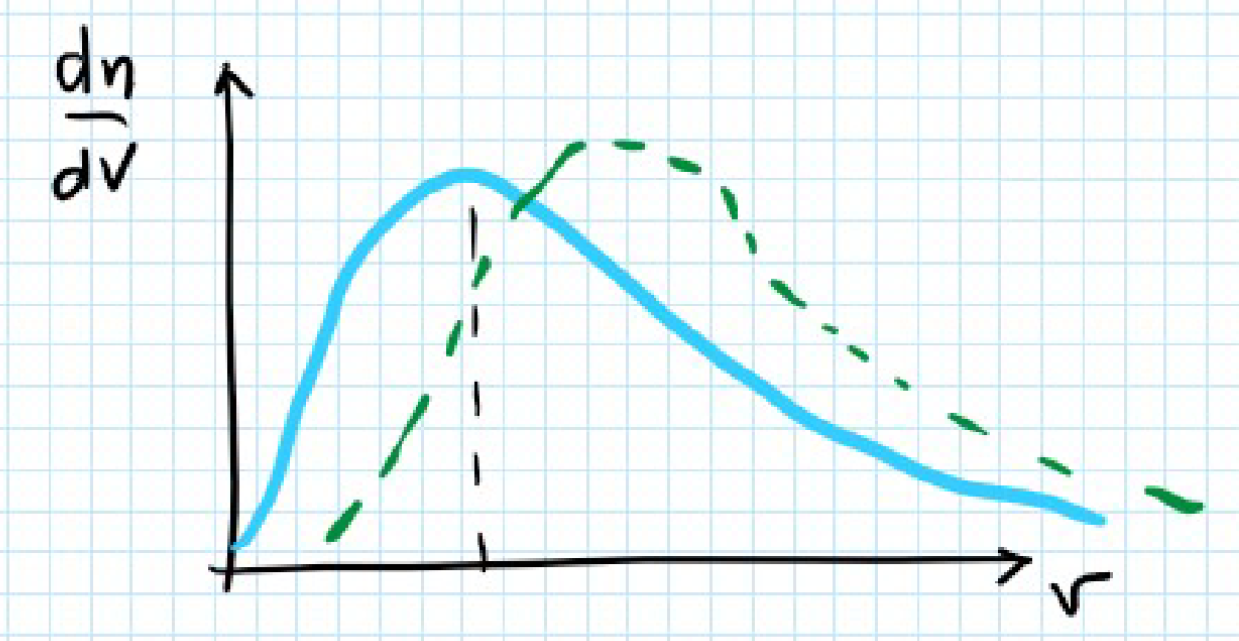
\includegraphics[width=9cm]{images/Distribuzione_Maxwell_Boltzmann.png}
    \caption{Distribuzione di Maxwell-Boltzmann. La curva verde corrisponde alla distribuzione per una temperatura maggiore rispetto a quella per la curva azzurra.}
\end{figure}
\end{definition}
\noindent
\`E possibile misurare se effettivamente la distribuzione \`e questa:
si fa girare una ruota velocemente con un buchino e poi si mettono a contatto la ruota con un tubo da cui esce il gas. Vedendo quante particelle sono arrivate sulle varie parti interne della ruota uno pu\`o capire la distribuzione.

\begin{figure}[!htb]
    \centering
    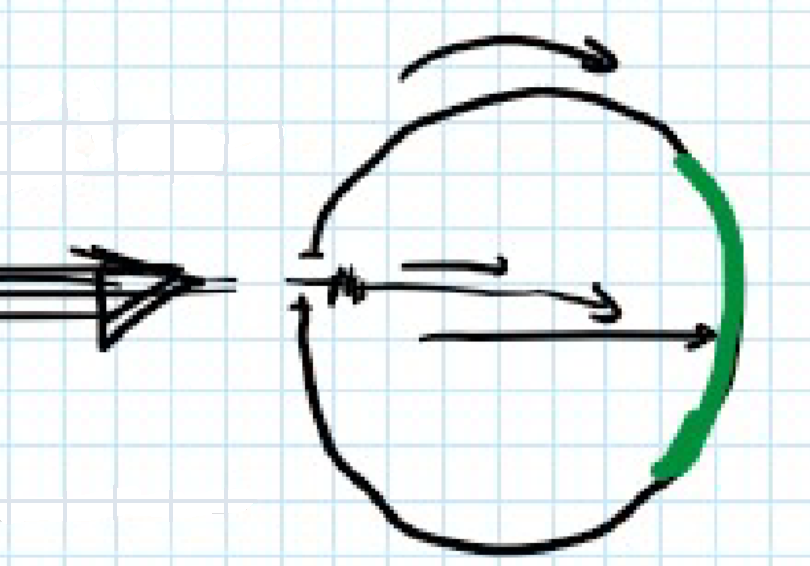
\includegraphics[width=7cm]{images/Misura_distribuzione_Maxwell_Boltzmann.png}
\end{figure}


\section{Entropia nel modello statistico}
\begin{definition}[Macro- e Microstati]
Dato un sistema statistico come quello trattato in questo capitolo, un \textbf{microstato} \`e il dato di ogni singola posizione e velocit\`a, un \textbf{macrostato} \`e la classe di microstati con le stesse propriet\`a globali (per esempio volume, temperatura, pressione).
\end{definition}
\begin{fact}
\textbf{Tutti i microstati compatibili con un dato macrostato sono equiprobabili.}
\end{fact}

\begin{remark}
Consideriamo due sistemi. Uno in un macrostato con probabilit\`a $P_1$ di verificarsi ed entropia $S_1$, il secondo con dati analoghi $P_2$ e $S_2$. Notiamo che l'insieme dei due sistemi ha entropia $S_1+S_2$ e la probabilit\`a del macrostato di questo insieme \`e $P_1P_2$. Intuitivamente abbiamo notato che
\[S\propto \log P\propto \log\Omega,\]
dove $\Omega$ \`e il numero di microstati con lo stesso macrostato.
\end{remark}

\begin{definition}[Entropia di Boltzmann]
Per una qualche costante\footnote{che troveremo in seguito} $C$ definiamo l'\textbf{entropia di Boltzmann} di un sistema come
\[S=C\log\Omega\]
\end{definition}

\noindent Proviamo a confrontare l'entropia di Boltzmann con quella che abbiamo gi\`a definito per alcune trasformazioni di gas ideali.

\subsection{Mescolamento dello stesso gas}

Consideriamo una scatola adiabatica con due compartimenti di volume $V/2$. Dentro il primo compartimento si trovano $r$ moli di gas e nel secondo $1-r$ moli, entrambi alla stessa temperatura. Rimuoviamo successivamente la parete e attendiamo l'equilibrio termodinamico.
\bigskip

\noindent La variazione di entropia termodinamica \`e
\begin{align*}
\Delta S=&(S_{f_1}-S_{i_1})+(S_{f_2}-S_{i_2})=\\
=&rR\log\pa{\frac{rV}{V/2}}+(1-r)R\log\pa{\frac{(1-r)V}{V/2}}=\\
=&R\pa{r\log r+(1-r)\log(1-r)+\log 2}.
\end{align*}
\noindent
Consideriamo ora l'entropia di Boltzmann:\\
Nel primo compartimento abbiamo $N/2 -x$ particelle e nel secondo $N/2 +x$.
\[\Omega(N,x)=\binom{N}{x+N/2},\]
da cui
\[S_i=C(\log(N!)-\log((N/2-x)!)-\log((N/2+x)!)).\]
Applicando l'approssimazione di Stirling $\log(N!)\simeq N\log N$ si ha
\[S_i\simeq -NC\pa{\pa{\frac12-\frac xN}\log\pa{\frac12-\frac xN}+\pa{\frac12+\frac xN}\log\pa{\frac12+\frac xN}}.\]
Riscrivendo questo risultato in termini di moli $r=\frac1{N_a}\pa{\frac{N_a}2-x}=\frac12-\frac x{N_a}$, si ha
\[S_i\simeq -N_a C\pa{r\log r+(1-r)\log (1-r)}\]
Per quanto riguarda lo stato finale il numero di microstati possibili ora \`e ogni combinazione di particelle nei due contenitori, $2^{N_a}$ possibilit\`a in totale, dunque
\[S_f=CN_a\log 2,\]
dunque
\[\Delta S=S_f-S_i=N_aC\pa{r\log r+(1-r)\log(1-r)+\log 2}.\]
\bigskip

\noindent Notiamo che le due espressioni sono la stessa se $C=k_b$, dunque troviamo la definizione di entropia di Boltzmann pi\`u conosciuta
\[\boxed{S=k\log \Omega}\]

\subsection{Espansione isoterma}
Fissiamo la temperatura e consideriamo una espansione da $V$ a $V+dV$. Ci aspettiamo che $\Omega$ cambi come segue
\[\frac{\Omega_f}{\Omega_i}=\frac{(V+dV)^N}{V^N}=\pa{1+\frac{dV}V}^N\]
Poich\'e stiamo considerando il modello di gas perfetto si ha che $dT=0\implies dU=0$, dunque
\[dV=\frac{\delta Q}p,\]
da cui
\[\frac{dV}V=\frac{\delta Q}{pV}=\frac{\delta Q}{nRT}=\frac{\delta Q}{Nk_b T}\]
Quindi l'entropia di Boltzmann verifica la definizione di entropia che avevamo dato per trasformazioni reversibili:
\[\Delta S=k_b\log\pa{\frac{\Omega_f}{\Omega_i}}=k_b N\log\pa{1+\frac{\delta Q}{Nk_b T}}\approx k_bN\frac{\delta Q}{Nk_bT}=\frac{\delta Q}T.\]

\subsection{Isocora}
Consideriamo ora una isocora e cambiamo la temperatura. Poich\'e
\[\ps{E_K}=\frac32k_bT\]
si ha che in ogni direzione 
\[\frac12m\ps{v_x^2}=\frac12 k_bT\implies \ps{v_x^2}=\frac{k_bT}m,\]
inoltre per isotropia $\ps{v_x}$, quindi $\sqrt{\frac{k_bT}m}$ \`e la deviazione standard di $v_x$.
Quindi $v$ per una particella ha una deviazione standard nell'ordine di $\pa{\frac{k_bT}m}^{3/2}$ quindi nell'insieme si ha che $\ps{v}\propto T^{3N/2}$.
\medskip

\noindent
Tornando alla trasformazione isocora abbiamo trovato che 
\[\frac{\Omega_f}{\Omega_i}=\pa{1+\frac{dT}T}^{3N/2},\]
da cui nuovamente
\[\Delta S=\frac{3N}2k_b\log\pa{1+\frac{dT}T}\approx \frac{3Nk_b}2\frac{dT}T=\frac{C_VdT}T=\frac{dU}T\pasgnl={isocora}\frac{\delta Q}T.\]



\section{Informazione}
\begin{definition}[Informazione]
Sia $X$ una variabile aleatoria discreta che pu\`o assumere $N$ valori $x_1,\cdots, x_N$ con densit\`a di probabilit\`a $P_i$. 
Definiamo l'\textbf{informazione} derivante dal fatto che l'evento $x_i$ sia accaduto come
\[I_i=-\log P_i\]
\end{definition}

\noindent
Vogliamo definire una funzione $\Hc(\cpa{P_i})$ che rappresenta ``l'informazione che manca per capire l'esito data una distribuzione di probabilit\`a". Imponiamo alcune propriet\`a:
\begin{itemize}
\item $\Hc$ deve essere continua nelle $P_i$
\item Se per ogni $P_i=\frac1N$, $\Hc$ deve essere monotona e crescente\footnote{Pi\`u esiti possibili corrisponde a pi\`u informazione necessaria per identificare l'evento accaduto} in $N$.
\item [(Consistenza)\ $\bullet$] Sia $\pi$ una partizione di $N$ e per ogni elemento $g\in \pi$ sia $P_g=\sum_{i\in g}P_i$, allora\footnote{$P(a\mid b)$ indica la probabilit\`a che accada $a$ dato che accade $b$, equivalentemente \[P(a\mid b)=P(a\wedge b)/P(b)\]}
\[\Hc(\cpa{P_i})=\Hc(\cpa{P_g}_{g\in \pi})+\sum_{g\in \pi} P_g\Hc(\cpa{P(x_i\mid g)})\]
\end{itemize}

\begin{theorem}[Entropia di Shannon]
La funzione $\Hc$ deve assumere la forma
\[\Hc(\cpa{P_i})=-C\sum_i P_i\log(P_i).\]
Questa funzione di dice \textbf{entropia di Shannon/Gibbs}.
\end{theorem}
\begin{proof}
Consideriamo due casi possibili per la distribuzione di probabilit\`a:
\setlength{\leftmargini}{0cm}
\begin{itemize}
\item[$\boxed{\text{uniforme}}$] Sia $\Hc(\cpa{N\ii,\cdots, N\ii})=F(N)$. Consideriamo ora $n$ collezioni di eventi equiprobabili. Ogni collezione $g$ contiene $N/n$ eventi, quindi $P_g=\frac1n$ e $P(x_i\mid g)=\frac nN$. Osserviamo dunque che $\Hc(\cpa{P(x_i\mid g)})=F(N/n)$. Per consistenza
\[F(N)=F(n)+\sum_n\frac1nF(N/n)=F(n)+F(N/n).\] 
Siano ora $s,t>1$ interi positivi e notiamo che esistono $\al,\beta$ interi con $\beta$ arbitrariamente grande tali che
\[\frac\al\beta\leq\frac{\log s}{\log t}<\frac{\al+1}\beta\implies t^\al\leq s^\beta<t^{\al+1}.\]
Per monotonia di $F$
\[F(t^\al)\leq F(s^\beta)<F(t^{\al+1}).\]
Per la propriet\`a di $F$ mostrata sopra si ha che
\[F(t^\al)=F(t)+F(t^{\al-1})=\cdots=\al F(t)\]
e similmente per gli altri termini, dunque
\[\frac\al\beta\leq\frac{F(s)}{F(t)}<\frac{\al+1}\beta.\]
Questo mostra che
\[\abs{\frac{F(s)}{F(t)}-\frac{\log s}{\log t}}\leq \frac1\beta,\]
e poich\'e $\beta$ pu\`o essere scelto grande a piacere questo mostra che $F(s)=C\log s$ per una qualche costante $C$.
\item[$\boxed{\text{generale}}$] Sia $N_g=\#g$. Notiamo che $P_g=\frac{N_g}N$ e che $P(x_i\mid g)=\frac1{N_g}$. Osserviamo che
\[\Hc(\cpa{P_i})=F(N)=\Hc(\cpa{P_g})+\sum_g P_g F(N_g),\]
da cui
\begin{align*}
\Hc(\cpa{P_g})=& F(N)-\sum_g P_g F(N_g)=\sum_g P_g(F(N)-F(N_g))=\\
=& C\sum_g P_g\log(N/N_g)=\\
=&-C\sum_g P_g\log(P_g).
\end{align*}
\end{itemize}
\setlength{\leftmargini}{0.5cm}
\end{proof}

\begin{remark}
L'entropia \`e la media pesata del logaritmo delle probabilit\`a nella distribuzione a meno di costante.
\end{remark}

\begin{remark}
Se $P_i=1/N$ allora \[\Hc(\cpa{P_i})=-C\sum_i \frac1N\log\frac1N=-C\log N,\]
che a meno della notazione \`e l'equivalente di $S=k_b\log \Omega$.
\end{remark}


\subsection{Principio di massima entropia}
\begin{fact}[Principio di massima entropia]
I sistemi tendono alla distribuzione che massimizza l'entropia compatibile con i vincoli.
\end{fact}

\subsubsection{Nessun vincolo}
Consideriamo un sistema con $N$ stati e nessun vincolo. Sia $P_i$ la probabilit\`a dello stato $i$. Vogliamo trovare i $P_i$ che massimizzano $S$ sapendo che $\sum_i P_i=1$:\\
Cerchiamo le soluzioni del sistema di moltiplicatori di Lagrange
\[\begin{cases}
\sum_i P_i=1\\
\pp{P_i}{}(-k_b\sum_j P_j\log P_j)=\la \pp{P_i}{}(-1+\sum_j P_j)
\end{cases}\]
\[\begin{cases}
\sum_i P_i=1\\
-k_b (\log P_i+1)=\la
\end{cases}\coimplies\begin{cases}
\sum_i P_i=1\\
P_i=e^{-\pa{\frac \la{k_b}+1}}
\end{cases}\]
Poich\'e $e^{-\pa{\frac \la{k_b}+1}}$ non dipende da $i$, il sistema ha come soluzione $P_i=N\ii$ per ogni $i$, dunque in assenza di vincoli
\[S=-k_b\sum_i\frac1N\log\pa{\frac1N}=k\log N.\]

\subsubsection{Un vincolo}
Consideriamo un vincolo della forma 
\[\ps{f(x_i)}\doteqdot\sum_i P_i f(x_i)=c.\]
Applicando nuovamente il sistema dei moltiplicatori di Lagrange ricaviamo\footnote{$f$ non dipende dalle probabilit\`a, quindi $\pp{P_i}f(x_i)=0$}
\[\begin{cases}
\sum_j P_j=1\\
\sum_j P_j f(x_j)=c\\
-k_b (\log P_i+1)=\al+\beta f(x_i)
\end{cases}\coimplies \begin{cases}
\sum_j P_j=1\\
\sum_j P_j f(x_j)=c\\
P_i=e^{-1-\al/k_b}e^{-(\beta/k_b) f(x_i)}
\end{cases}\]
Applicando la prima equazione troviamo
\[e^{-1-\al/k_b}\under{\doteqdot Z}{\pa{\sum_j e^{-(\beta/k_b)f(x_j)}}}=1,\]
da cui
\[P_i=\frac1Ze^{-\frac\beta{k_b}f(x_i)}.\]
Inserendo questa scrittura nella formula per l'entropia di Shannon troviamo
\begin{align*}
S=&-k_b\sum_i \frac1Ze^{-\frac\beta{k_b}f(x_i)}\log\pa{\frac1Ze^{-\frac\beta{k_b}f(x_i)}}=\\
=&k_b\log Z-k_b\sum_i P_i\log\pa{e^{-\frac\beta{k_b}f(x_i)}}=\\
=&k_b\log Z+\beta\ps{f(x_i)} 
\end{align*}

\begin{example}[Energia interna costante]
Sia $f(x_i)=E(x_i)$ e supponiamo che $U=\ps{E}$ sia costante. L'entropia \`e della forma
\[S=k_b\log Z+\beta U\]
Poich\'e $Z$ \`e costante, $\beta=\pp US=\frac1T$, dunque
\[S=k_b\log Z+\frac UT.\]
Osserviamo inoltre che per quanto detto
\[P_i=\frac1Z \exp\pa{-\dfrac{E(x_i)}{k_bT}},\]
che a meno della costante di normalizzazione $Z$ corrisponde ad un termine che appare nella distribuzione di Maxwell-Boltzmann.
\end{example}